\section{Συστήματα διαλόγου}
Ως \newterm{Σύστημα Διαλόγου}{Dialogue System}
ή \newtermsee{Διαδραστικό Πράκτορα Ομιλίας}{Interactive Conversational Agent}{Σύστημα Διαλόγου - Dialogue System}
ή \en{chatterbot / chatbot}
ορίζουμε ένα σύστημα σχεδιασμένο να αλληλεπιδρά με έναν χρήστη χρησιμοποιώντας φυσική γλώσσα.

\begin{figure}
    \centering
    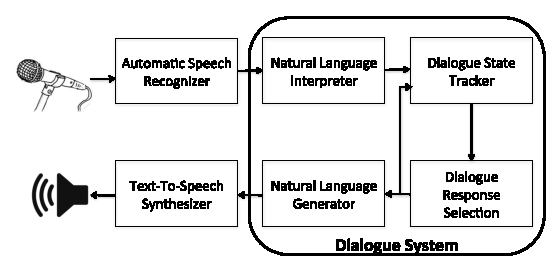
\includegraphics{dialogue-system-diagram}
    \ccaption{Ένα σύστημα διαλόγου}{serban2015survey}
    \label{fig:dialogue-system-diagram}
\end{figure}

Σε αντίθεση με τους στόχους αυτής της διπλωματικής, τα συστήματα διαλόγου χαρακτηρίζονται από μεγαλύτερη αλληλεπίδραση με τον χρήστη.
Τους δίνεται η δυνατότητα να θέτουν ερωτήσεις για την επίλυση πιθανών απροσδιοριστιών και έχουν τη δυνατότητα να δίνουν απαντήσεις σε ερωτήματα του χρήστη.
Ωστόσο, μερικές βασικές αρχές και μέθοδοι που εφαρμόζονται στη βιβλιογραφία μπορούν να χρησιμοποιηθούν και στο πλαίσιο αυτής της εργασίας.

Ένας πιθανός διαχωρισμός των διάφορων συστημάτων διαλόγου γίνεται σύμφωνα με τον σκοπό χρήσης τους:
στα \newtermprint[Goal-driven Dialogue Systems]{Συστήματα Διαλόγου Προσανατολισμένα για Καθήκοντα}
και στα \newtermprint[Non-goal-driven Dialogue Systems]{Συστήματα Διαλόγου που δεν είναι Προσανατολισμένα για Καθήκοντα}.
Ωστόσο, ο διαχωρισμός αυτός δεν είναι πάντα αυστηρός και μερικά συστήματα μπορεί να συνδυάζουν χαρακτηριστικά και από τις δύο κατηγορίες~\cite{wang2016recent}.

\subsection{Συστήματα διαλόγου που δεν είναι προσανατολισμένα για καθήκοντα}\label{subsec:non-goal-driven-dialogue-systems}%
\index{Σύστημα Διαλόγου - Dialogue System!Μη Προσανατολισμένα για Καθήκοντα - Non-goal-driven}
Αποτελούν μοντέλα που δεν έχουν έναν συγκεκριμένο σκοπό και προσπαθούν να διεξάγουν διάλογο προσομοιώνοντας έναν ανθρώπινο συνομιλητή.
Παραδείγματα χρήσεων αποτελούν η εκμάθηση γλώσσας ή απλώς η διασκέδαση~\cite{shawar2007chatbots,serban2015hierarchical}.

Ένα από τα πρώτα συστήματα διαλόγου ήταν η ELIZA~\cite{weizenbaum1966eliza} που προσπαθούσε να προσομοιώσει τις απαντήσεις ενός ψυχοθεραπευτή σε μια ψυχιατρική συνέντευξη.
Η ELIZA όμως δεν είχε κάποιον τρόπο να ακολουθεί τη συζήτηση ή να απαντάει σύμφωνα με το παρελθόν.
Έχει θεωρηθεί~\cite{shieber1994lessons} ότι η αρχική επιτυχία που είχε η ELIZA μπορεί να αποδοθεί στο ότι οι άνθρωποι μπορούν εύκολα να ξεγελαστούν αποδίδοντας δομή στο χάος, δίνοντας σημασία εκεί που δεν υπάρχει.
Στην ίδια κατεύθυνση, ένα άλλο σύστημα διαλόγου, ο PARRY~\cite{colby1981modeling}, προσπαθούσε να μιμηθεί τη συμπεριφορά ενός παρανοϊκού ασθενούς.
Το σύστημα ήταν ανώτερο καθώς είχε επίγνωση του ιστορικού της συζήτησης και της κατάστασης του μυαλού του.
Ωστόσο, όπως και η ELIZA, ο PARRY δεν έβγαζε συμπεράσματα ούτε \enquote{σκεφτόταν} την απάντησή του αλλά αναγνώριζε κάποια πρότυπα στην είσοδό του~\cite{colby1974ten}.
Κανένα από αυτά τα δύο συστήματα δεν χρησιμοποιούσε προσεγγίσεις μηχανικής μάθησης.

Αργότερα~\cite{shawar2007chatbots,serban2015survey}, εμφανίστηκαν συστήματα με διαφορετικές αρχιτεκτονικές.
Ένα από τα πρώτα που χρησιμοποιούσε μηχανική εκμάθηση είναι το \lib{MegaHal}~\cite{hutchens1998introducing} που αναπτύχθηκε για την εισαγωγή του στον διαγωνισμό \lib{Loebner}.
Μοντελοποιούσε τον διάλογο ως στοχαστική ακολουθία διακριτών συμβόλων με Μαρκοβιανές αλυσίδες.
Οι πιθανές απαντήσεις του \lib{MegaHal} βασίζονταν στην επιλογή λέξεων-κλειδιών από την είσοδο του χρήστη.
Αφού παρήγαγε αρκετές απαντήσεις, επέλεγε αυτή που προσέφερε την περισσότερη πληροφορία -- μεγαλύτερη εντροπία.
Το σύστημα άρχιζε με μηδενική γνώση της γλώσσας και εκπαιδευόταν σε έναν συνδυασμό πηγών:
\begin{compactitem}
    \item Προτάσεις που περιείχαν ένα φτιαχτό όνομα, ηλικία, απασχόληση και προσπαθούσαν να δώσουν \enquote{χαρακτήρα} στον \lib{MegaHal}
    \item Εγκυκλοπαιδικές γνώσεις
    \item Διάλογοι από ταινίες και σειρές
    \item Γνωστά αποσπάσματα
    \item Μερικά κείμενα σε γλώσσες διάφορες της αγγλικής
\end{compactitem}

Στην ίδια περίοδο, οι~\citet{levin1997stochastic} και \citet{levin1998using} πρότειναν για πρώτη φορά τη χρήση \newterm{Διαδικασ\rr{ιών}{ίες} Απόφασης Μάρκοβ}{Markov Decision Process - MDP}
και αργότερα αναπτύχθηκαν αρκετά συστήματα βασισμένα σε αυτές.
Για παράδειγμα, το RLDS~\cite{singh2000reinforcement}, ένα γενικό εργαλείο για συστήματα διαλόγου,
και το ELVIS~\cite{walker1998learning}, μια \newterm{Διεπαφή Ομιλούμενης Γλώσσας}{Spoken Language Interface - SLI} για την πρόσβαση σε μηνύματα ηλεκτρονικού ταχυδρομείου μέσω τηλεφώνου.
Στη συνέχεια, έγινε ιδιαίτερα διαδεδομένη~\cite{young2013pomdp,wang2016recent,roy2000spoken,young2002talking} η χρήση
\newtermc[Διαδικασίες Απόφασης Μάρκοβ - Markov Decision Process - MDP]{\rr{μ}{Μ}ερικώς \rr{π}{Π}αρατηρήσιμ\rr{ων}{ες} \dd{διαδικασιών απόφασης Μάρκοβ}}{Partially Observable \dd{Markov Decision Process} - POMDP}
στην οποία θεωρείται ότι ο διάλογος εξελίσσεται ως μια διαδικασία Μάρκοβ: ξεκινώντας από κάποια αρχική κατάσταση $s_0$, κάθε επόμενη κατάσταση διαμορφώνεται από μια πιθανότητα μετάβασης.
Το μοντέλο εκπαιδεύεται στα δεδομένα για να μάθει την καλύτερη πολιτική διαλόγου.

Πιο σύγχρονα συστήματα διαλόγου εφαρμόζουν μοντέλα που βασίζονται σε αρχιτεκτονικές που αξιοποιούν νευρωνικά δίκτυα αλλά αυτά απαιτούν τη χρήση μεγάλου πλήθους δεδομένων για την εκπαίδευσή τους~\cite{serban2015survey}.
Σε αυτά περιλαμβάνονται τα \newtermprint[end-to-end]{άκρη-προς-άκρη} μοντέλα~\cite{serban2015survey,serban2016building}
που αντί να υλοποιούν ένα σύστημα πολλών τμημάτων με ξεχωριστές λειτουργίες,
εκπαιδεύονται ως ένα ενιαίο μοντέλο - \enquote{μαύρο κουτί} - στις εισόδους και τις εξόδους του επιθυμητού συστήματος διαλόγου.

\subsection{Συστήματα διαλόγου προσανατολισμένα για καθήκοντα}\label{subsec:goal-driven-dialogue-systems}%
\index{Σύστημα Διαλόγου - Dialogue System!Προσανατολισμένα για Καθήκοντα - Goal-driven}
Αυτά τα μοντέλα συνήθως αξιοποιούν τεχνικές για τη μοντελοποίηση του διαλόγου παρόμοιες με αυτές των συστημάτων διαλόγου που δεν είναι προσανατολισμένα για καθήκοντα αλλά,
επιπλέον, περιλαμβάνουν τη χρήση τεχνικών που σχετίζονται με την εκτέλεση κάποιας πράξης σύμφωνα με τις επιθυμίες του χρήστη.

Μια βασική μονάδα που συναντάται σε αυτά τα συστήματα και μας ενδιαφέρει για την υλοποίηση αυτής της διπλωματικής είναι αυτό της
\newterm{Κατανόηση\dd{ς} Φυσικής Γλώσσας}{Natural Language Understanding - NLU}.
Στόχο της αποτελεί η αντιστοίχηση του κειμένου σε νόημα, δηλαδή η παραγωγή μιας σημασιολογικής αναπαράστασης ενός κειμένου~\cite{martin2009speech}.

\subsubsection{Προθέσεις και οντότητες}\label{subsec:intents-and-entities}
\begin{figure}
    \centering
    \begin{tabular}{|lcccccccc|}
        \hline
        \textbf{Λέξεις}       & book                                       & flight       & from         & Thessaloniki & to           & Reykjavík    & this         & weekend      \\
                              & $\downarrow$                               & $\downarrow$ & $\downarrow$ & $\downarrow$ & $\downarrow$ & $\downarrow$ & $\downarrow$ & $\downarrow$ \\
        \textbf{Slots}        & \noslot{}                                  & \noslot{}    & \noslot{}    & B-departure  & \noslot{}    & B-arrival    & B-date       & I-date       \\
        \textbf{Entity Types} & \noslot{}                                  & \noslot{}    & \noslot{}    & B-city       & \noslot{}    & B-city       & B-date       & I-date       \\
        \textbf{Intent}       & \multicolumn{8}{l|} {\intent{book_flight}}                                                                                                          \\
        \hline
    \end{tabular}
    \lcaption{Παράδειγμα αναγνώρισης πρόθεσης και εξαγωγής οντοτήτων}{%
        Η επισήμανση γίνεται με τη μορφή \newterm{Εσωτερικό-Εξωτερικό-Έναρξη}{Inside–Outside–Beginning - IOB}.
        Οι οντότητες \engquote{Thessaloniki} και \engquote{Reykjavík} έχουν τον ίδιο τύπο, αυτό της πόλης,
        αλλά πληρούν διαφορετικά σημασιολογικά ορίσματα στην πρόθεση: η πρώτη αποτελεί την τοποθεσία αναχώρησης και η άλλη την τοποθεσία άφιξης.%
    }%
    \label{fig:ex-intent-entity}
\end{figure}
Η πρώτη βασική διεργασία της NLU στα συστήματα διαλόγου προσανατολισμένα για καθήκοντα είναι
η \newterm{Αναγνώριση Πρόθεσης}{Intent Identification} ή \newtermsee{Ταξινόμηση Πρόθεσης}{Intent Classification}{Αναγνώριση Πρόθεσης - Intent Identification}
του χρήστη.
Μια πρόθεση είναι ένας σκοπός ή ένας στόχος που υποδηλώνεται από τα λεγόμενα του χρήστη,
αποτελεί μια παράγωγη σημασιολογική αναπαράσταση των λεγόμενων του χρήστη.
Για παράδειγμα, στην πρόταση \enquote{What's the weather like in Thessaloniki?} ο στόχος του χρήστη είναι να μάθει την κατάσταση του καιρού.
Στη διαδικασία της αναγνώρισης, το σύστημα ταξινομεί τα λεγόμενα του χρήστη σε μια ή περισσότερες προκαθορισμένες προθέσεις και εξάγει τις σχετικές οντότητες.
Συνήθως, οι προκαθορισμένες προθέσεις σχεδιάζονται από εμπειρογνώμονες σύμφωνα με τον τομέα της εφαρμογής
και τα συστήματα εκπαιδεύονται πάνω σε επισημασμένα σύνολα δεδομένων~\cite{tur2005semi}.

Συγγενικό στόχο με την αναγνώριση πρόθεσης αποτελεί η \newterm{Εξαγωγή Οντοτήτων}{Entity Extraction} και η \newterm{Πλήρωση Υποδοχέων}{Slot Filling}.
Αν και μερικές φορές οι δύο όροι χρησιμοποιούνται ως ισοδύναμοι,
οι υποδοχείς λειτουργούν ως σημασιολογικά ορίσματα που το μοντέλο καλείται να καλύψει ώστε να προσδιοριστούν οι λεπτομέρειες της πρόθεσης του χρήστη
ενώ οι οντότητες χαρακτηρίζονται από κλάσεις και παίρνουν τιμές άσχετα με την πρόθεση μέσα στην οποία εμφανίζονται~\cite{mesnil2013investigation,snips} (βλέπε και~\fref{fig:ex-intent-entity}).
Το ζητούμενο εδώ είναι η εκχώρηση μιας σημασιολογικής έννοιας σε κάθε λέξη της πρότασης~\cite{vu2016bi}.
Για παράδειγμα, στην πρόταση \engquote{What's the weather like in Thessaloniki?} η λέξη \engquote{Thessaloniki} πρέπει να επισημανθεί ως η πόλη για την οποία ο χρήστης θέλει να μάθει τον καιρό.
Οι οντότητες συνδέονται στενά με τις προκαθορισμένες προθέσεις που αναγνωρίζει το σύστημα, τροποποιούν και προσδιορίζουν κάθε μια από αυτές, αποτελούν σημασιολογικούς προσδιοριστές.
Οι υπόλοιπες λέξεις που δεν συνδέονται με κάποια αναγνωρισμένη σημασιολογική έννοια επισημαίνονται με μία κενή κλάση, \noslot{}.

Οι δύο αυτοί στόχοι αποτελούν ακόμη μια δύσκολη πρόκληση για την ερευνητική κοινότητα~\cite{tur2011intent,sarikaya2017technology}.

Η αναγνώριση πρόθεσης συνήθως υλοποιείται με μεθόδους ταξινόμησης κειμένου, κυρίως με μεθόδους μάθησης με επίβλεψη.
Βασικό πρόβλημα αποτελεί η ανάγκη μεγάλου αριθμού επισημασμένων δεδομένων των οποίων η έλλειψη είναι ιδιαίτερα φανερή σε καινούργιους κλάδους~\cite{wang2016recent}.
Συναντώνται υλοποιήσεις που χρησιμοποιούν
τον αλγόριθμο Boosting~\cite{schapire2000boostexter},
\newterm{Μηχανές Διανυσμάτων Υποστήριξης}{Support Vector Machines - SVM}~\cite{haffner2003optimizing,bhargava2013easy},
\newterm{Ταξινομητές Μέγιστης Εντροπίας}{Maximum Entropy Classifiers}~\cite{ang2005automatic} και
μοντέλα λογιστικής παλινδρόμησης~\cite{snips,rasa}.
Σε πιο σύγχρονες δημοσιεύσεις, εμφανίζονται μέθοδοι βασισμένες σε νευρωνικά δίκτυα όπως:
\newterm[Νευρωνικά Δίκτυα]{Βαθιά Δίκτυα Πεποιθήσεων}{Deep Belief Networks - DBN}~\cite{sarikaya2014application},
\newterm[Νευρωνικά Δίκτυα]{Συνελικτικά\dd{ Νευρωνικά Δίκτυα}}{Convolutional\dd{ Neural Networks} - CNN}~\cite{kim2014convolutional,zhang2015sensitivity},
συνδυασμός CNN με \newterm[Νευρωνικά Δίκτυα]{\dd{Δίκτυα }Μακράς Βραχυπρόθεσμης Μνήμης}{Long Short-Term Memory - LSTM}~\cite{zhou2015c} και
\newterm[Νευρωνικά Δίκτυα]{Ανατροφοδοτούμενα\dd{ Νευρωνικά Δίκτυα}}{Recurrent\dd{ Neural Networks} - RNN}~\cite{yang2016hierarchical},

Οι βασικές παραδοσιακές προσεγγίσεις για την εξαγωγή οντοτήτων βασίζονται σε
\newtermprint[Hidden Markov Models - HMM]{Κρυφά Μαρκοβιανά Μοντέλα}~\cite{wang2005spoken} και
CRF~\cite{raymond2007generative,wang2011semantic,wang2016recent,rasa,snips}.
Πιο πρόσφατα, έχουν επίσης χρησιμοποιηθεί RNN~\cite{mesnil2013investigation,yao2013recurrent,mesnil2015using,liu2015recurrent,vu2016bi} και LSTM~\cite{yao2014spoken} δίκτυα.

Η ανάθεση σημασιολογικών ρόλων (\SRLR{}) έχει εμφανισθεί και στη βιβλιογραφία των συστημάτων διαλόγου.
Οι \citet{tur2005semi} χρησιμοποίησαν SRL για την \newtermprint[clustering]{Ομαδοποίηση} προτάσεων χρηστών που δεν είχαν κατηγοριοποιηθεί σύμφωνα με την πρόθεσή τους.
Από τα δεδομένα εκπαίδευσης εξάγονται τα πιο συχνά εμφανιζόμενα ζευγάρια δομών κατηγορημάτων-ορισμάτων και από αυτά ένας ειδικός καλείται να δημιουργήσει κανόνες που μεταφράζουν τις δομές αυτές σε προθέσεις.
Στο~\cite{chen2013unsupervised} επιχειρείται η αυτόματη εξαγωγή και πλήρωση σημασιολογικών υποδοχέων ακατέργαστων ηχητικών δεδομένων για την επιτάχυνση της διαδικασίας δημιουργίας συστήματος διαλόγου ομιλίας.

\subsubsection{Κοινά μοντέλα}
Στη βιβλιογραφία προτείνονται \newtermprint[Joint Models]{Κοινά Μοντέλα}
που στοχεύουν στην ταυτόχρονη επίλυση των προβλημάτων της αναγνώρισης προθέσεων και εξαγωγής οντοτήτων.
Η λογική αυτών των προσεγγίσεων βασίζεται στο ότι υπάρχει ισχυρή στατιστική διασύνδεση των δύο αυτών διεργασιών.
Αποτελούν προσεγγίσεις που προσπαθούν να συνδυάσουν την επισήμανση μιας ακολουθίας κειμένου με την ταξινόμησή της.
Δηλαδή, το μοντέλο πρέπει να καταχωρεί μια ετικέτα σε κάθε στοιχείο της ακολουθίας και να ταξινομεί την ακολουθία ως σύνολο με μια κλάση ή ετικέτα.
Μια προσέγγιση που αναφέρεται στη βιβλιογραφία είναι τα
\newtermc[Υπό Συνθήκη Τυχαίο Πεδίο - Conditional Random Field - CRF]{\rr{τ}{Τ}ριγωνικ\rr{ά CRF}{ό}}{Triangular\dd{ CRF} - TriCRF}~\cite{jeong2008triangular}
που επεκτείνουν τη λειτουργία των γραμμικών \CRFR{} χρησιμοποιώντας μια επιπλέον μεταβλητή που εκφράζει την πρόθεση της πρότασης εισόδου.
Στο~\cite{xu2013convolutional} προτάθηκε μια έκδοση των TriCRF με CNN όπου τα χαρακτηριστικά που χρησιμοποιούνται εξάγονται από τις βαθμίδες του νευρωνικού δικτύου.
Επίσης, έχουν χρησιμοποιηθεί LSTM δίκτυα~\cite{hakkani2016multi,zhou2016hierarchical}.

Τέλος, μερικές προσεγγίσεις προσπαθούν να αξιοποιήσουν την επιτυχία της \newterm[Νευρωνικά Δίκτυα]{Μεταφορά\dd{ς} Μάθησης}{Transfer Learning} σε άλλα προβλήματα,
όπως στον τομέα της μηχανικής όρασης~\cite{sharif2014cnn,girshick2014rich,donahue2014decaf}.
Η πρόσφατη δημοτικότητα δημοσιεύσεων που σχετίζονται με έννοιες μεταφοράς μάθησης όπως τα BERT~\cite{bert}, ELMO~\cite{elmo} και ULMFiT~\cite{ulmfit} στον κλάδο της επεξεργασίας φυσικής γλώσσας
καταδεικνύει ότι είναι πιθανό να εμφανιστούν αρκετές μελλοντικές εφαρμογές με μοντέλα που εκμεταλλεύονται τη μεταφορά πληροφορίας.
Στο~\cite{goyal2018fast} χρησιμοποιούνται
\newterm[Νευρωνικά Δίκτυα!Μακράς Βραχυπρόθεσμης Μνήμης - Long Short-Term Memory - LSTM]{Αμφίδρομα \dd{δίκτυα μακράς βραχυπρόθεσμης μνήμης}}{Bi-directional\dd{ LSTM Networks}}
που εκπαιδεύονται πρώτα σε σύνολα δεδομένων που περιέχουν μεγάλο αριθμό επισημασμένων προθέσεων και οντοτήτων και μετά προσαρμόζουν το δίκτυο σε ένα καινούργιο σύνολο δεδομένων με μικρότερο αριθμό παραδειγμάτων.

\subsubsection{Multi-intent detection}\label{subsec:multi-intent}
Στα περισσότερα σύγχρονα συστήματα διαλόγου προσανατολισμένα για καθήκοντα, θεωρείται ότι για κάθε είσοδο ή πρόταση του χρήστη υπάρχει μόνο μια πρόθεση.
Το υποπρόβλημα της
\newterm[Αναγνώριση Πρόθεσης - Intent Identification]{Αναγνώριση\dd{ς} Πολλαπλών Προθέσεων}{Multi-Intent / Multiple Intent Identification}
ανά πρόταση είναι ένας τομέας με συγκριτικά λίγες σχετικές δημοσιεύσεις.
Για παράδειγμα, στην πρόταση \engquote{Move forwards while waving hand} πρέπει να ανιχνευθούν οι προθέσεις \intent{BodyMotion} και \intent{ArmMotion}.
Τέτοιου τύπου προτάσεις μπορούν να δυσχεράνουν μοντέλα που είναι εκπαιδευμένα σε δεδομένα που περιέχουν αποκλειστικά \newtermprint[Single Intent]{μονές προθέσεις} ανά πρόταση.

Οι \citet{xu2013exploiting} προσπαθούν να επιλύσουν το πρόβλημα χρησιμοποιώντας κατηγοριοποίηση πολλών ετικετών.
Ωστόσο, το μοντέλο τους απαιτεί την εκπαίδευση πάνω σε δεδομένα με προτάσεις που περιέχουν πολλαπλές προθέσεις χρηστών.
Αυτό αυξάνει σημαντικά τις απαιτήσεις για δεδομένα εκπαίδευσης.
Επίσης, οι πιθανές προθέσεις ανά πρόταση περιορίζονται σε δύο και οι συνδυασμοί τους θεωρούνται ως ξεχωριστή ετικέτα,
για παράδειγμα \intent{buy_game+play_game}.

Οι \citet{kim2017two} επιχειρούν την ανίχνευση πολλαπλών προθέσεων σε δύο στάδια.
Στο πρώτο, η πρόταση χωρίζεται σε πιθανές υποθέσεις σύμφωνα με τους \newterm{\rr{συνδέσμους}{Σύνδεσμος}}{Conjunction} που περιέχονται στην πρόταση.
Για παράδειγμα, η πρόταση \engquote{Record Phineas and Ferb and play OCN news} παράγει δύο υποθέσεις:
\begin{compactenum}
    \item \engquote{Record Phineas and Ferb} \textbf{and} \engquote{play OCN news}
    \item \engquote{Record Phineas} \textbf{and} \engquote{Ferb and play OCN news}
\end{compactenum}
όπου, προφανώς, ο πρώτος διαχωρισμός είναι ο επιθυμητός.
Σε κάθε υπόθεση δίνεται η ίδια βαθμολογία με την ελάχιστη βαθμολογία των προθέσεων που την αποτελούν.
Επιλέγεται η υπόθεση με τη μέγιστη βαθμολογία.
Το δεύτερο στάδιο κυρίως αφορά προτάσεις στις οποίες
η \newtermprint[Automatic Speech Recognition - ASR]{Αυτόματη Αναγνώριση Ομιλίας}
αποτυγχάνει να αναγνωρίσει τους απαραίτητους συνδέσμους και η αναγνώριση των πολλαπλών προθέσεων γίνεται μέσω μιας προσέγγισης επισήμανσης ακολουθίας.
Ένα πλεονέκτημα αυτής της προσέγγισης είναι η έλλειψη της ανάγκης ύπαρξης δεδομένων εκπαίδευσης που να περιέχουν πολλές προθέσεις ανά πρόταση.
Το πρώτο στάδιο χρησιμοποιεί μοντέλα εκπαιδευμένα μόνο σε μονές προθέσεις ανά πρόταση
ενώ το δεύτερο χρησιμοποιεί μια μέθοδο αυτόματης παραγωγής κατάλληλων δεδομένων με πολλαπλές προθέσεις ανά είσοδο.
Ένας σημαντικός περιορισμός είναι ότι λειτουργεί με την προϋπόθεση ότι ο μέγιστος αριθμός προθέσεων ανά πρόταση είναι δύο.
Επίσης, η μέθοδος που ακολουθείται αδυνατεί να αναλύσει επιτυχώς πιο περίπλοκες συντακτικές δομές όπως η ανύψωση δεξιού κόμβου (βλέπε \fref{subsec:linguistics}).

Η χρήση ενός \newtermprint[Hierarchical Model]{Ιεραρχικού Μοντέλου} προτείνεται από τους \en{\citet{rychalska2018multi}}.
Αρχικά, πραγματοποιείται η κατηγοριοποίηση των \enquote{μεγάλων υποδοχών} (\en{Big Slots}) οι οποίες περιέχουν το τμήμα της πρότασης που περιλαμβάνει την πρόθεση του χρήστη.
Στη συνέχεια, πραγματοποιείται η κατηγοριοποίηση των λεπτομερειών --- \enquote{μικρών υποδοχών} (\en{Small Slots}) --- με βάση τα χαρακτηριστικά της μεγάλης υποδοχής στην οποία εμπεριέχεται η μικρή.
Δοκιμάζεται ένα μοντέλο με CRF και ένα με δίκτυα GRU-RNN.
Για τους σκοπούς της εκπαίδευσης δημιουργήθηκε μια βάση δεδομένων που αποτελείται από προτάσεις που ενίοτε περιέχουν πολλαπλές προθέσεις.

Οι \citet{xia2018zero} προτείνουν, χωρίς να έχουν υλοποιήσει, την εύρεση πολλαπλών προθέσεων μέσω του διαχωρισμού τους σε απλές προθέσεις και την επισήμανση αυτών με εργαλεία ακολουθιακής κατηγοριοποίησης όπως τα CRF.
Ένα πιθανό πρόβλημα με αυτή την προσέγγιση είναι ότι είναι δυνατή η επικάλυψη των προθέσεων μέσα σε μια πρόταση.
Δηλαδή, μια λέξη μιας πρότασης θα μπορούσε να ανήκει ταυτόχρονα σε παραπάνω από μια πρόθεση.
Μια λύση σε αυτό το πρόβλημα θα μπορούσε να είναι η χρήση μοντέλων πολλών ετικετών.

\subsubsection{Υλοποιήσεις σε βιβλιοθήκες λογισμικού ανοιχτού κώδικα}
\ig[type=pdf,inc={width=\linewidth}]{snips}{\lcaption{Μονάδα NLU του \lib{Snips}}{%
        Συνδυάζονται δύο προσεγγίσεις για την αναγνώριση της πρόθεσης~\protect\cite{snips}.
        Ο \newtermprint[Deterministic Intent Parser]{Ντετερμινιστικός Αναλυτής Πρόθεσης}
        δημιουργεί κανόνες κανονικών εκφράσεων έτσι ώστε να είναι σίγουρη η σωστή ταξινόμηση των παραδειγμάτων που συναντώνται στο σύνολο εκπαίδευσης.
        Ο \newtermprint[Probabilistic Intent Parser]{Πιθανοτικός Αναλυτής Πρόθεσης}
        αποτελείται από ένα μοντέλο λογιστικής παλινδρόμησης για την αναγνώριση πρόθεσης και ένα γραμμικό CRF για τις οντότητες κάθε πρόθεσης.
        Δηλαδή, αφού αναγνωρισθεί η πρόθεση, το αντίστοιχο CRF καλείται να εξάγει τις οντότητες του δοθέντος κειμένου.

        Τέλος, οι τιμές των οντοτήτων μετατρέπονται από φυσική γλώσσα σε τιμές του μεγέθους που μετράνε μορφοποιημένες σύμφωνα με ISO.
        Για παράδειγμα, το \engquote{tomorrow} θα μετατραπεί σε μορφή \en{\texttt{YYYY-MM-DD hh:mm:ss}}.
        Για την εξαγωγή των οντοτήτων χρησιμοποιείται η βιβλιοθήκη \libcite{Rustling} που αποτελεί μια εκ νέου υλοποίηση της βιβλιοθήκης \libcite[Python!]{Duckling}.%
    }%
}
Το \libcite[Python!]{Snips} αποτελεί μια πλατφόρμα που στοχεύει στη δημιουργία ψηφιακών βοηθών που αλληλεπιδρούν φωνητικά με τον χρήστη.
Χρησιμοποιεί μια \newtermprint[Software Pipeline]{σωλήνωση λογισμικού}, που παρουσιάζεται στο \fref{fig:snips}, για την υλοποίηση της μονάδας κατανόησης φυσικής γλώσσας%
\footnote{Ο κώδικας της μονάδας βρίσκεται στο \url{https://github.com/snipsco/snips-nlu}}.
Στη δημοσίευση αιτιολογείται η επιλογή των CRF αντί για τα μοντέλα RNN των~\cite{mesnil2013investigation,mesnil2015using} διότι είναι υπολογιστικά πιο ελαφριά με παρόμοιες ωστόσο αποδόσεις.
Παρόλα αυτά, χρήσιμη θα ήταν η διερεύνηση της χρήσης νεότερων μοντέλων από πιο πρόσφατες δημοσιεύσεις.

Στο \libcite[Python!]{RASA} προσφέρεται ένα ζευγάρι εργαλείων
για την κατανόηση φυσικής γλώσσας\footnote{Ο κώδικας βρίσκεται στο \url{https://github.com/RasaHQ/rasa}}
και για τη διαχείριση διαλόγου\footnote{Ο κώδικας βρίσκεται στο \url{https://github.com/RasaHQ/rasa_core}}.
Η πρώτη αποτελεί μια βιβλιοθήκη που προσφέρει διάφορες μονάδες σχετικές με την κατανόηση και επεξεργασία φυσικής γλώσσας.
Στόχος είναι η δημιουργία μιας σωλήνωσης λογισμικού σύμφωνα με τις προτιμήσεις του χρήστη / προγραμματιστή.
Ως προεπιλογή για την αναγνώριση πρόθεσης, χρησιμοποιείται ένα γραμμικό SVM πολλών κλάσεων με τη βοήθεια της βιβλιοθήκης \libcite[Python!]{scikit-learn}.
Ως είσοδος μπορούν να δοθούν \newterm{Διανύσματα Λέξεων}{Word Vectors} όπως παράγονται από το \libcite{GloVe} ή οποιαδήποτε άλλη μέθοδο αναπαράστασης λέξεων με αριθμητικά διανύσματα.
Εναλλακτικά, μπορεί να γίνει χρήση ενός μοντέλου νευρωνικών δικτύων, με τη βοήθεια του \libcite[Python!]{Tensorflow},
που βασίζεται στην ιδέα από το \lib{StarSpace}~\cite{wu2018starspace} και επιτρέπει την αναγνώριση πολλαπλών προθέσεων αν ο προγραμματιστής συμπεριλάβει δεδομένα για κάθε επιθυμητό συνδυασμό προθέσεων.
Για την εξαγωγή προκαθορισμένων οντοτήτων όπως απόσταση και ημερομηνίες υπάρχει και εδώ μονάδα που χρησιμοποιεί τη βιβλιοθήκη \libcite[Python!]{Duckling}.
Για μη-προκαθορισμένες οντότητες που εισάγει ο προγραμματιστής γίνεται χρήση CRF.

Το \libcite[Python!]{DeepPavlov} αποτελεί μια βιβλιοθήκη που χρησιμοποιεί τεχνικές βαθιάς μάθησης για τη δημιουργία συστημάτων διαλόγων προσανατολισμένων και μη για καθήκοντα.
Προσφέρονται διεπαφές για τη χρήση διάφορων αρχιτεκτονικών νευρωνικών δικτύων και είναι η δυνατή η χρήση των ELMO~\cite{elmo} και BERT~\cite{bert}.

% vim:ts=4:sw=4:expandtab:fo-=tc:tw=120
